\section{Descrizione architettura}
% Nell'indice proposto da Tullio c'è:
% a. Metodo e formalismo di specifica
% b. Presentazione dell'architettura generale del sistema e identificazione dei componenti architetturali di alto livello

\subsection{Metodo e formalismo di specifica}

Le scelte progettuali per lo sviluppo di \ProjectName{} sono state fortemente influenzate dallo stack tecnologico utilizzato.

In primo luogo il progetto è basato su Node.js ed è scritto quindi in JavaScript: un linguaggio che è (tra le altre caratteristiche) orientato agli oggetti (\glossario{OOP}), ma che lascia grande libertà al programmatore nella scelta della tecnica da utilizzare per l'implementazione di pattern come l'\glossario{incapsulamento} e l'\glossario{ereditarietà}. Al contrario di altri linguaggi (C++, Java) non c'è un costrutto esplicito con il quale il programmatore può definire classi. 

Progettare il sistema con un'architettura ad oggetti classica non permette di rappresentare in modo immediato la gestione dinamica dei tipi e le caratteristiche tipiche degli stili di programmazione funzionali. In certi casi è stato necessario introdurre interfacce ``fittizie'', che non verranno codificate. Dato che questo introduce numerosi schematismi che appesantiscono i diagrammi e che non sono richiesti dal linguaggio di programmazione, si è cercato di limitarli soltanto ai casi in cui sono particolarmente utili.

Il nostro approccio alla progettazione è stato contemporaneamente top-down e bottom-up. Da un lato siamo partiti suddividendo il sistema in front-end e back-end, definendo l'interfaccia di comunicazione, scegliendo di seguire in ciascuno l'organizzazione suggeritaci dai framework (Express e Angular.js). Dall'altro lato siamo partiti dal basso, componendo e cercando di riutilizzare il più possibile le librerie già esistenti. Per far questo abbiamo prima cercato e confrontato con attenzione la struttura e le scelte sia di progetti open source che di progetti proposti come best-practise.

L'approccio top-down è stato schematizzato nei diagrammi di deployment e dei package. Per la costruzione dei diagrammi delle classi, invece, questo approccio si è rivelato essere molto poco produttivo e rigoroso. I diagrammi delle classi proposti sono quindi \emph{uno dei possibili diagrammi} che descrivono l'applicazione, qualsiasi gerarchia o relazione complicata tra le classi verrebbe tradotta pressapoco nello stesso codice.

Per descrivere il sistema si è rivelato molto più comodo utilizzare i diagrammi di sequenza e di attività in un approccio bottom-up, descrivendo l'interazione tra i singoli oggetti senza preoccuparci della loro classificazione. In questo modo siamo anche riusciti a descrivere alcuni dei meccanismi tipici dell'applicazione, in particolar modo l'ordine in cui agiscono i \glossario{middleware} di Express. Riteniamo che saranno molto utili per la progettazione di dettaglio e per la codifica.

A posteriori, riteniamo che sarebbe stato molto meglio progettare il sistema seguendo uno stile di scomposizione modulare \emph{orientato alle funzioni}\footnote{Descritto alla sezione 11.3.2 del libro ``Ingegneria del software - Sommerville - 8a edizione (2007)''} o a flusso di dati piuttosto che \emph{a oggetti}. Con questa modifica radicale al metodo di specifica sarebbe stato possibile rappresentare in modo più naturale diverse delle caratteristiche salienti delle tecnologie e librerie utilizzate, che si strutturano meglio come pipeline piuttosto che come classi.

I diagrammi di deployment, dei \glossario{package}, delle classi, di sequenza e di attività presentati di seguito utilizzano la specifica \glossario{UML} 2.0.

\subsection{Architettura generale}

L'architettura del progetto si suddivide innanzitutto in una componente Client, costituita dal browser degli utenti che interagiranno con il \glossario{front-end} dell'applicazione, e in una componente WebServer, su cui verrà posto il \glossario{back-end}. Riguardo al server che ospita i database (la cui configurazione non è compito del progetto) non è necessario che risieda sullo stesso nodo su cui è posto il \glossario{back-end}.

\begin{figure}[H]
\centering
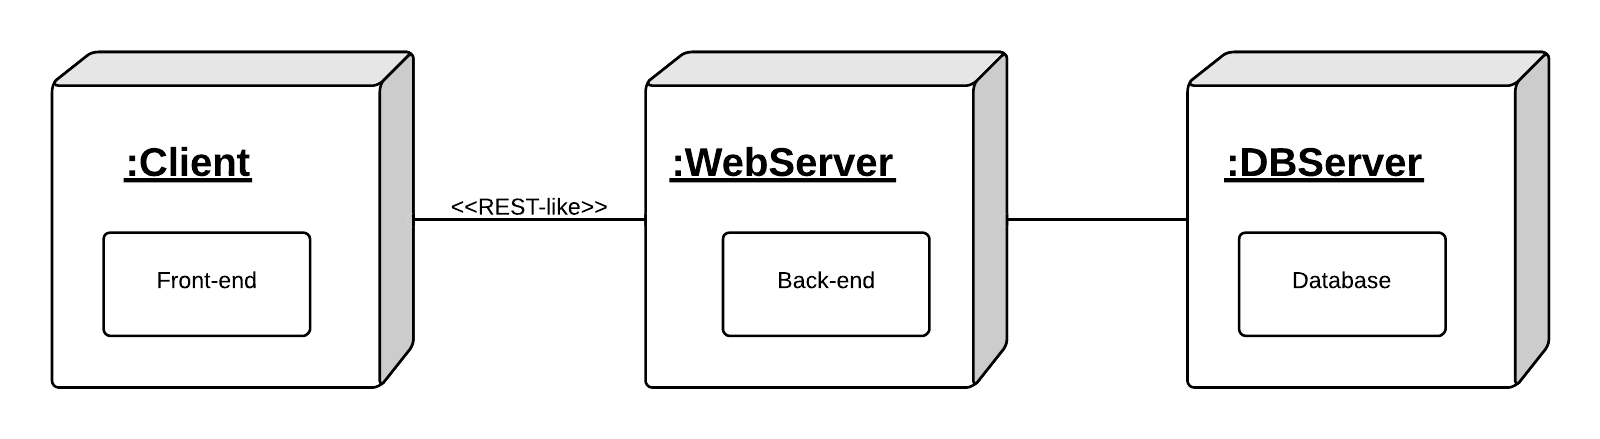
\includegraphics[width=\textwidth]{uml/diagramma-deployment.png}
\caption{Diagramma di deployment}
\end{figure}

\subsection{Interfaccia REST-like}
Per l'interfaccia della componente Back-end di \ProjectName{} si è scelto di utilizzare uno stile \glossario{REST-like}, ovvero basato sullo stile \glossario{REST} ma modificato per permettere l'autenticazione (tramite cookie) e l'attivazione di determinate operazioni. All'interno di un'unica sessione utente, a partire dall'operazione di login fino a quella di logout, l'interfaccia con cui si accede agli elementi delle collection può considerarsi effettivamente \glossario{REST}.

I motivi che hanno spinto alla scelta di \glossario{REST} sono:
\begin{itemize}
	\item Semplicità di utilizzo;
	\item Facile integrazione con i framework esistenti (Angular.js e Express);
	\item Indipendenza dal linguaggio di programmazione utilizzato;
\end{itemize}

\glossario{REST} utilizza il concetto di risorsa, ovvero un aggregato di dati con un nome (\glossario{URI}) e una rappresentazione, su cui è possibile invocare le operazioni \glossario{CRUD} tramite la seguente corrispondenza:

\begingroup
\renewcommand*{\arraystretch}{1.5}
\begin{tabularx}{\textwidth}{|P{2.5cm}|X|X|}
\hline
	\textbf{Risorsa} & \textbf{URI della collection} \newline es. http://example.com/users & \textbf{URI di un elemento} \newline es. http://example.com/users/42 \\
\hline
	\textbf{GET} & \textbf{Fornisce} informazioni sui membri della collection. & \textbf{Fornisce} una rappresentazione dell'elemento della collection indicato, espresso in un appropriato formato. \\
\hline
	\textbf{PUT} & Non usata. & \textbf{Sostituisce} l'elemento della collection indicato, o se non esiste, lo \textbf{crea}. \\
\hline
	\textbf{POST} & \textbf{Crea} un nuovo elemento nella collection. La URI del nuovo elemento è generata automaticamente ed è di solito restituita dall'operazione. & Non usato. \\
\hline
	\textbf{DELETE} & Non usata. & \textbf{Cancella} l'elemento della collection indicato. \\
\hline
\end{tabularx}
\endgroup

Per il formato di rappresentazione dei dati è stato scelto \glossario{JSON}, in quanto si integra molto facilmente con i framework utilizzati e con il linguaggio \glossario{JavaScript}, a differenza di \glossario{XML} o \glossario{CSV} che richiederebbero l'utilizzo di librerie specifiche.


\subsubsection{Back-end}

\begin{figure}[H]
\centering
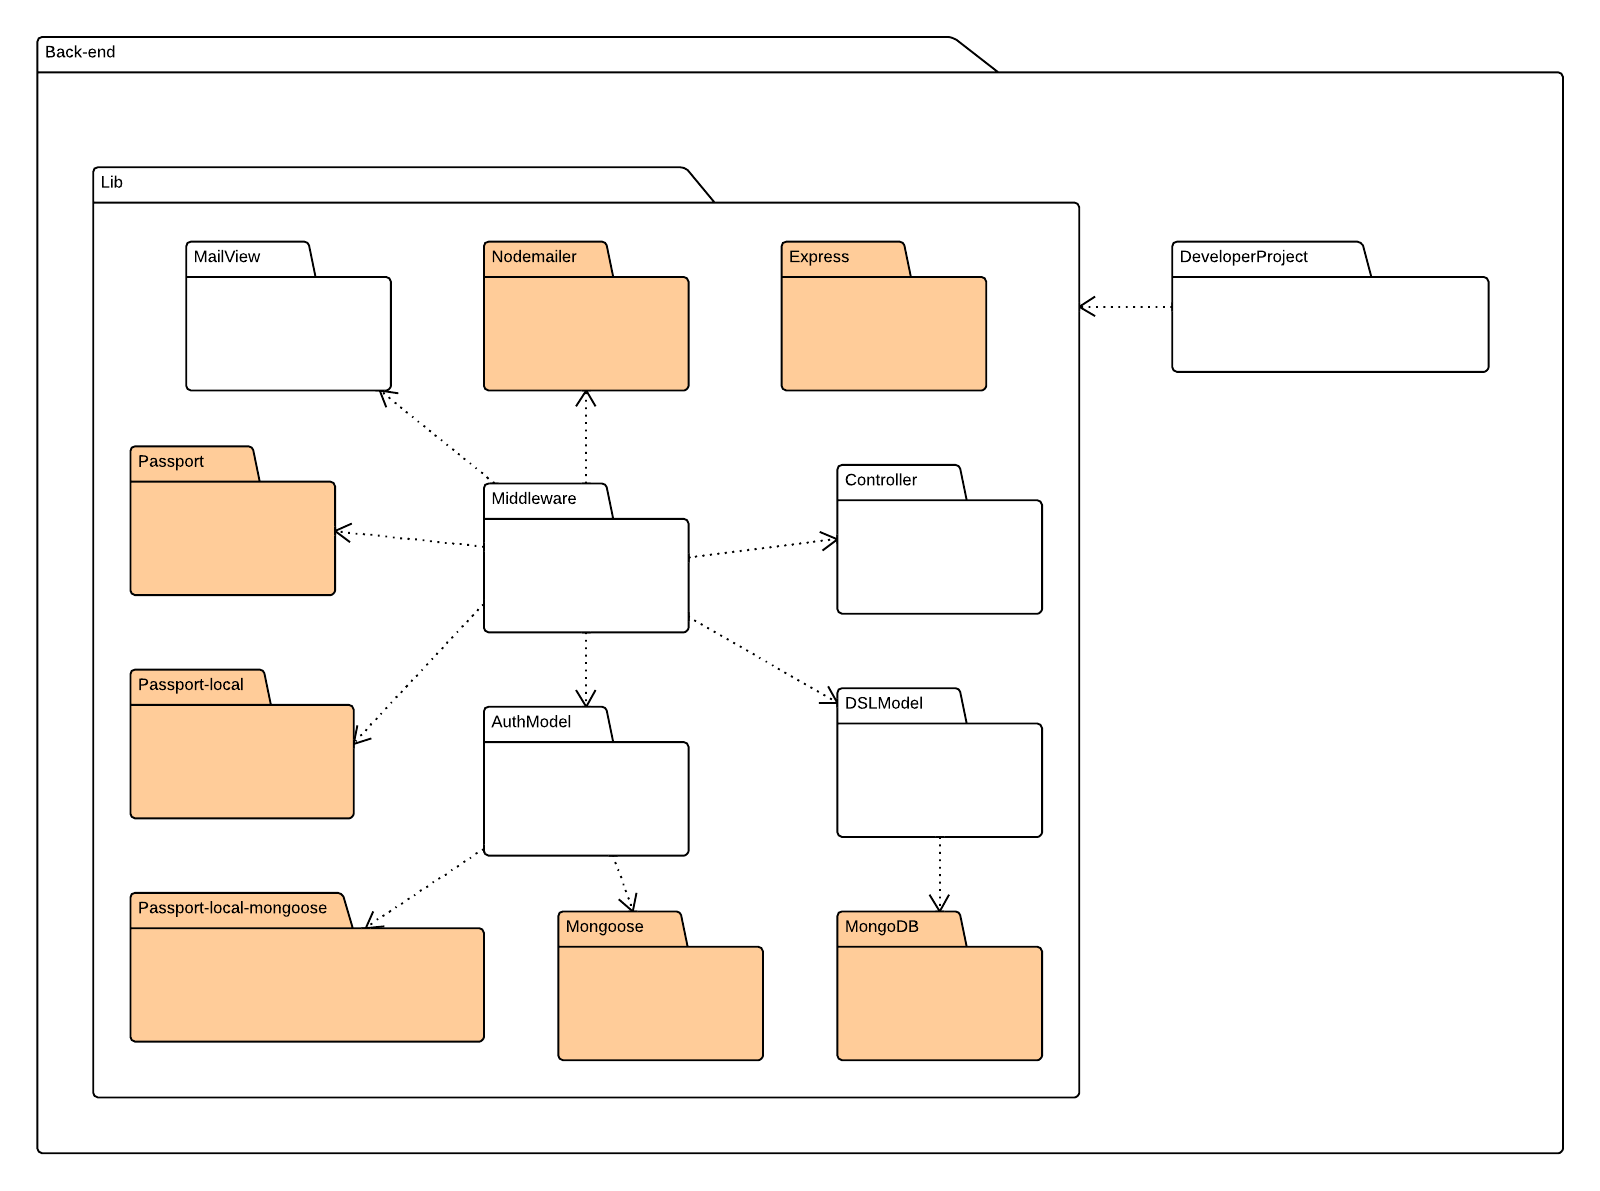
\includegraphics[width=\textwidth]{uml/Back-end-Diagramma dei Packages.png}
\caption{Diagramma dei package del Back-end}
\end{figure}

L'architettura del \glossario{back-end} si serve del pattern architetturale \glossario{MVC} (\textit{Model-View-Controller}), suddividendo i controller tradizionali dai controller \glossario{middleware}, come incoraggiato dal framework Express. Nei diagrammi non è rappresentata la \textit{view} poiché essa consiste nel \glossario{front-end}.

Il \glossario{front-end}, come descritto più avanti, utilizza anch'esso internamente un'architettura della famiglia \glossario{MVC}, ma dal punto di vista del \glossario{back-end} può considerarsi semplicemente una \textit{view}. La comunicazione tra i due avviene utilizzando il formato \glossario{JSON} e la conversione dalla rappresentazione interna alla presentazione testuale (\glossario{JSON}) è automatica e diretta. La struttura dati inviata, in particolare, coincide con la componente \textit{model} del front-end.

\subsubsection{Front-End}

\begin{figure}[H]
\centering
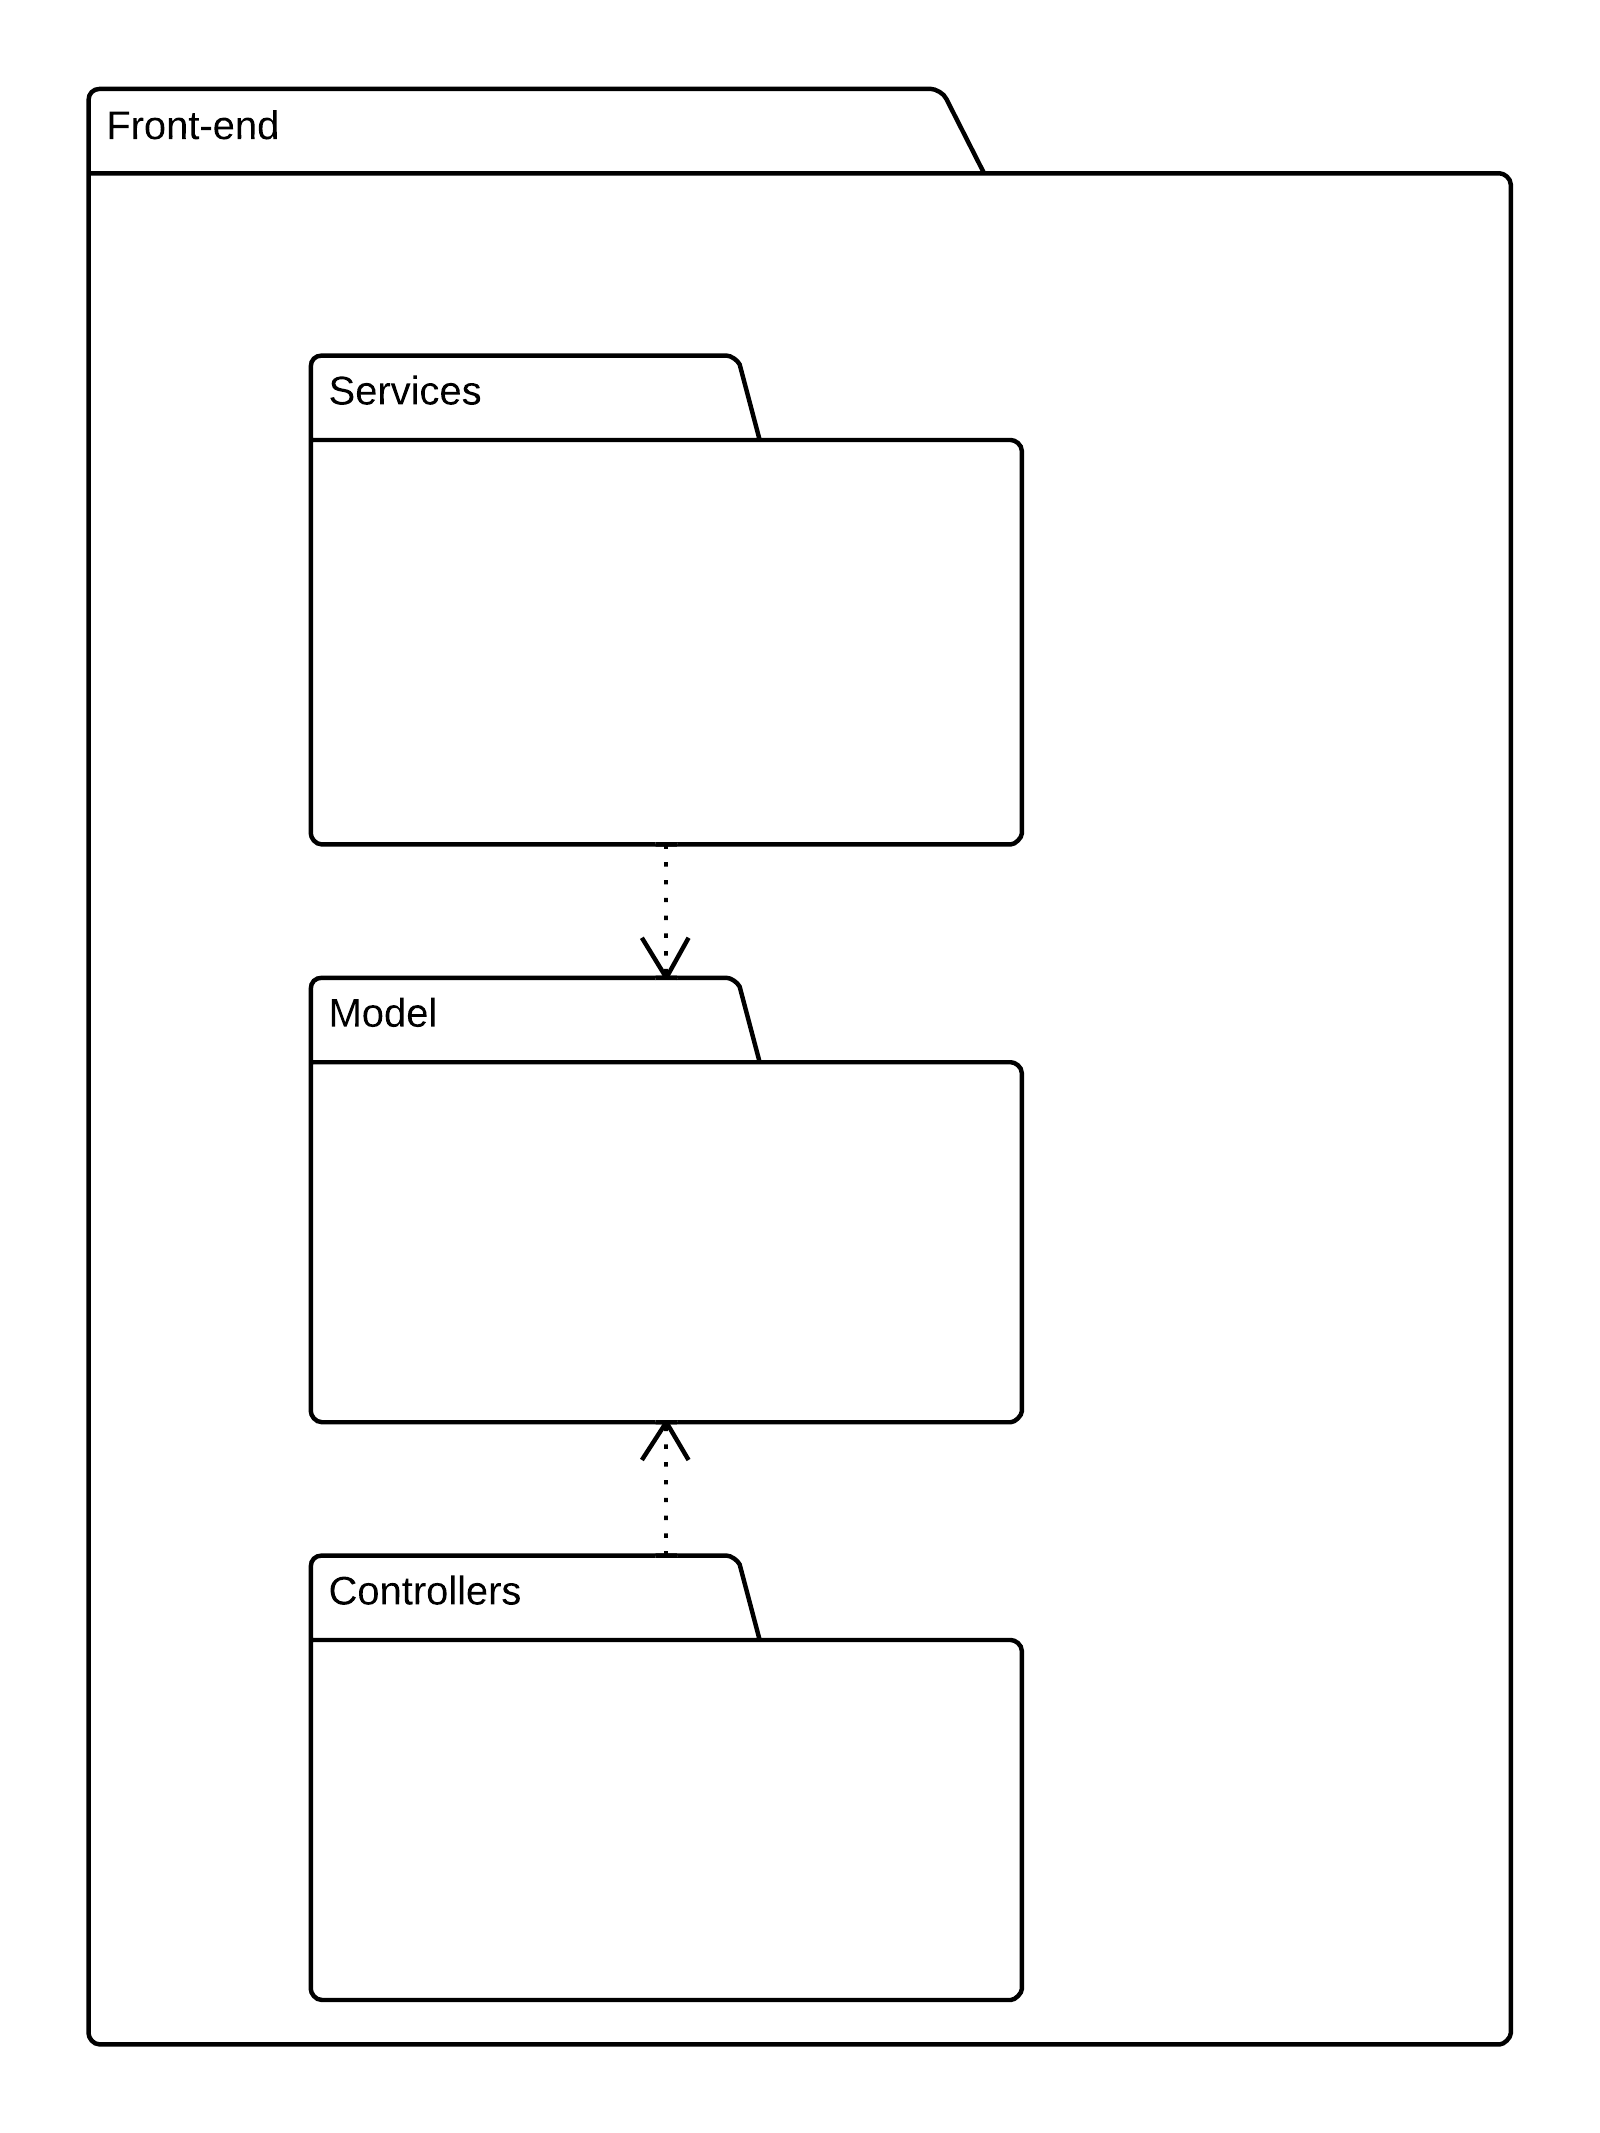
\includegraphics[width=0.5\textwidth]{uml/Front-end-Diagramma dei packages.png}
\caption{Diagramma dei package del Front-end}
\end{figure}

Il \glossario{front-end} è gestito dal \glossario{framework} \glossario{AngularJS}, la cui architettura è definita \glossario{MVW} (ossia \textit{Model-View-Whatever}) per la caratteristica di non corrispondere esattamente ad uno dei modelli classici. Nell'architettura si è scelto di descrivere i \glossario{package} del controller e del model, nonché un package che definisce i servizi con i quali i controller potranno interagire con il \glossario{back-end} e popolare i modelli di AngularJS. La view non è rappresentata poiché consiste unicamente in dei file statici di template scritti in un linguaggio molto simile all'\glossario{HTML}. Tali file risiedono fisicamente sul web-server, assieme alle librerie \glossario{JavaScript} e ad altri file statici; vengono caricati da \glossario{AngularJS} nel momento in cui il controller ne fa richiesta.